\documentclass[10pt,a4paper]{article}

\usepackage{polski}
\usepackage[utf8]{inputenc}

\usepackage[polish]{babel}
\usepackage{hhline}
\usepackage{pgfplots}

\usepackage{multicol}
%\usepackage{slashbox}
\usepackage{graphicx}
\usepackage{caption}
\usepackage{subcaption}
\usepackage{colortbl}

\usepackage{geometry}
\geometry{a4paper, total={170mm,257mm}, left=20mm, top=20mm }

\author{Sebastian Maciejewski 132275 i Jan Techner 132332}
\title{Badanie optycznych widm emisyjnych - \\ doświadczenie 304 (sala 221)}
\date{19 stycznia 2017}
\setlength{\parindent}{0pt}
\newcommand{\forceindent}{\leavevmode{\parindent=3em\indent}}
\begin{document}
\maketitle
\section{Wstęp teoretyczny}
\forceindent Widmo jest bardzo szerokim pojęciem w nauce i technice. W ogólnym znaczeniu jest to zależność natężenia sygnału od jego częstotliwości.
Widmo dotyczy również światła. Światłem powszechnie nazywamy fale elektromagnetyczne widzialne przez człowieka (długości fal z
zakresu $380 \pm 780 nm$). W technice światło jest pojęciem szerszym: są to fale elektromagnetyczne, które spełniają zasady optyki geometrycznej.
Do obserwacji i rejestracji widm w zakresie widzialnym używa się spektrometrów wyposażonych w elementy rozszczepiające światło (pryzmaty lub siatki dyfrakcyjne). 

\subsection*{Opis doświadczenia}
\forceindent Doświadczenie polega na analizowaniu widm uzyskiwanych dzięki spektrometrowi w programie komputerowym. Źródłem światła dla spektrometru
jest światłowód, którego koniec znajduje się na suwaku przed rzędem lamp - dzięki przesunięciu światłowodu przed wybraną lampę, program wyświetla
wykres natężenia światła od długości fali dla światła danej lampy.  

\section{Wyniki pomiarów}

\forceindent Na początek zajmijmy się widmem otrzymanym dzięki lampom A, B i C, aby ustalić pierwiastki zawarte w tych lampach. Poniżej znajduje się tabela z
obserwacjami.

\begin{center}
\begin{tabular}{|c|c|c|c|c|c|}
\multicolumn{2}{c}{Lampa A} & \multicolumn{2}{c}{Lampa B} & \multicolumn{2}{c}{Lampa C}\\
\hline
$\lambda (nm)$ & Natężenie & $\lambda (nm)$ & Natężenie & $\lambda (nm)$ & Natężenie\\
\hline
485,3 & b. małe & 387,8 & duże & 585,8 & b. duże\\
\hline
655,9 & duże & 446,5 & średnie & 594,3 & małe \\
\hline
750,3 & b. duże & 500,7 & duże & 609,3 & średnie \\
\hline
763,2 & średnie & 589,0 & b. duże & 614,3 & duże \\
\hline
810,9 & średnie & 667,3 & b. duże & 625,7 & małe \\
\hline
814,5 & małe & 706,2 & b. duże & 633,2 & małe \\
\hline
&& 728,2 & średnie & 639,9 & b. duże \\
\hline
&&&& 650,2 & średnie \\
\hline
&&&& 655,9 & małe \\
\hline
&&&& 667,3 & małe \\
\hline
&&&& 692,3 & b. małe \\
\hline
&&&& 703,3 & małe \\
\hline

\end{tabular}
\end{center}

\newpage
Następnym etapem doświadczenia była rejestracja widm lamp 1, 2 i 3 (dla różnych kolorów) oraz kilku widm lampy 4 dla różnych natężeń prądu. Otrzymane zostały następujące widma:\\

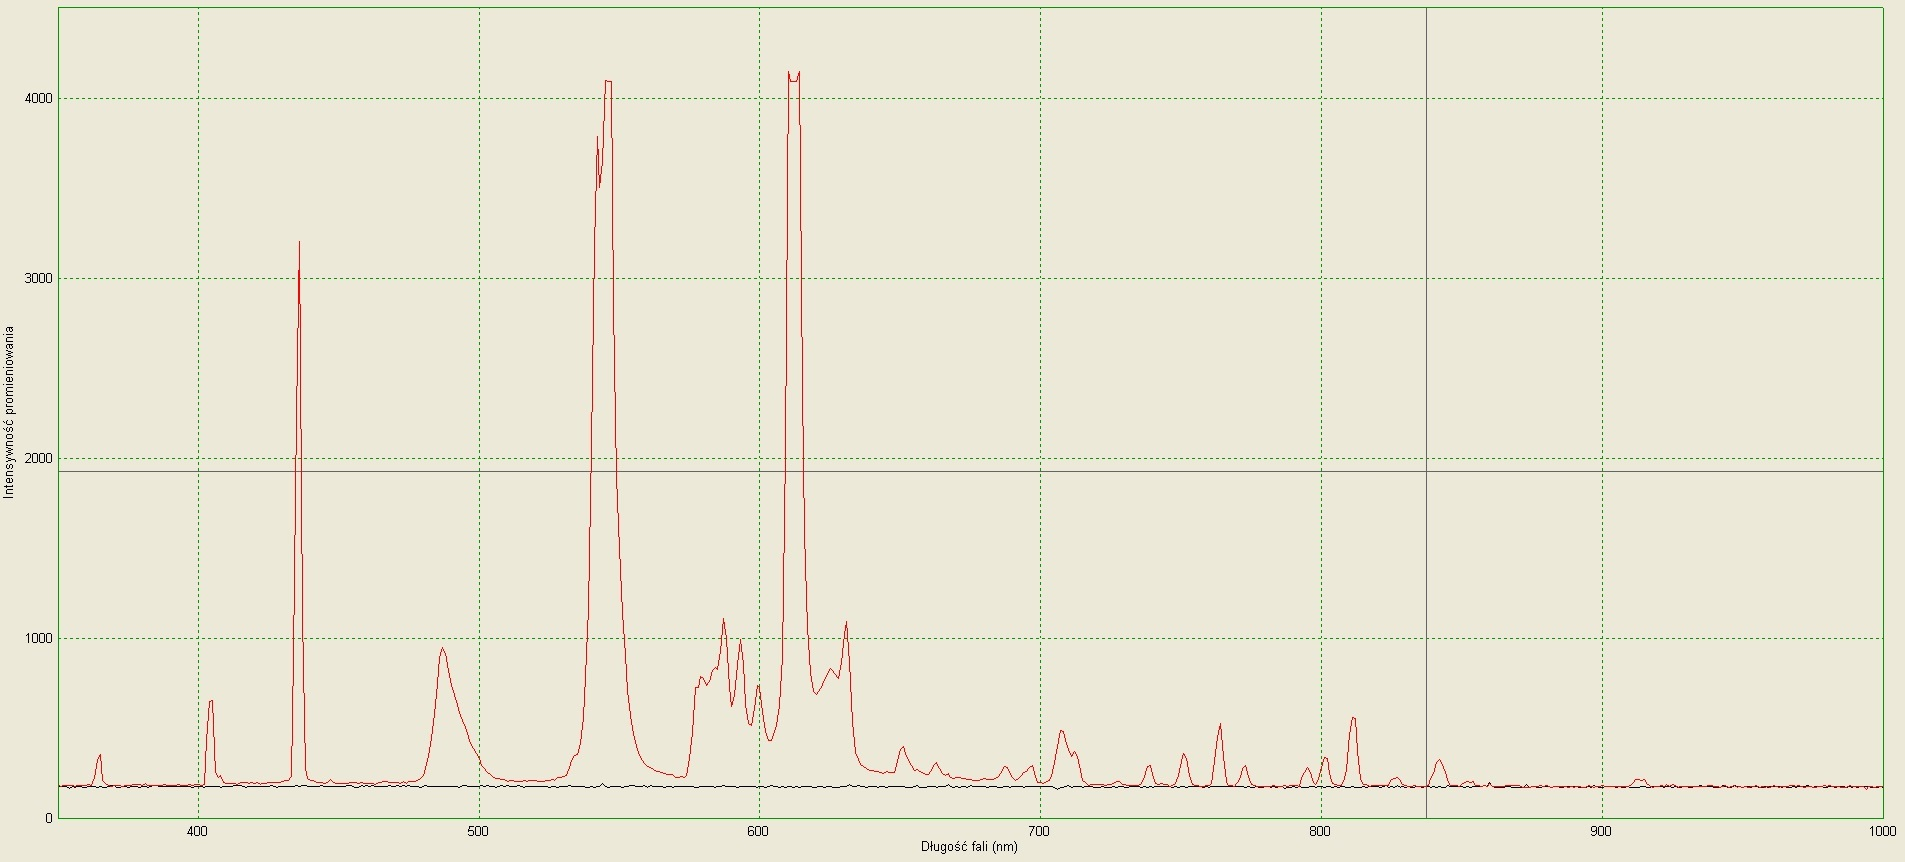
\includegraphics[width=\textwidth]{lampa1}
Widmo lampy 1.\\
\\
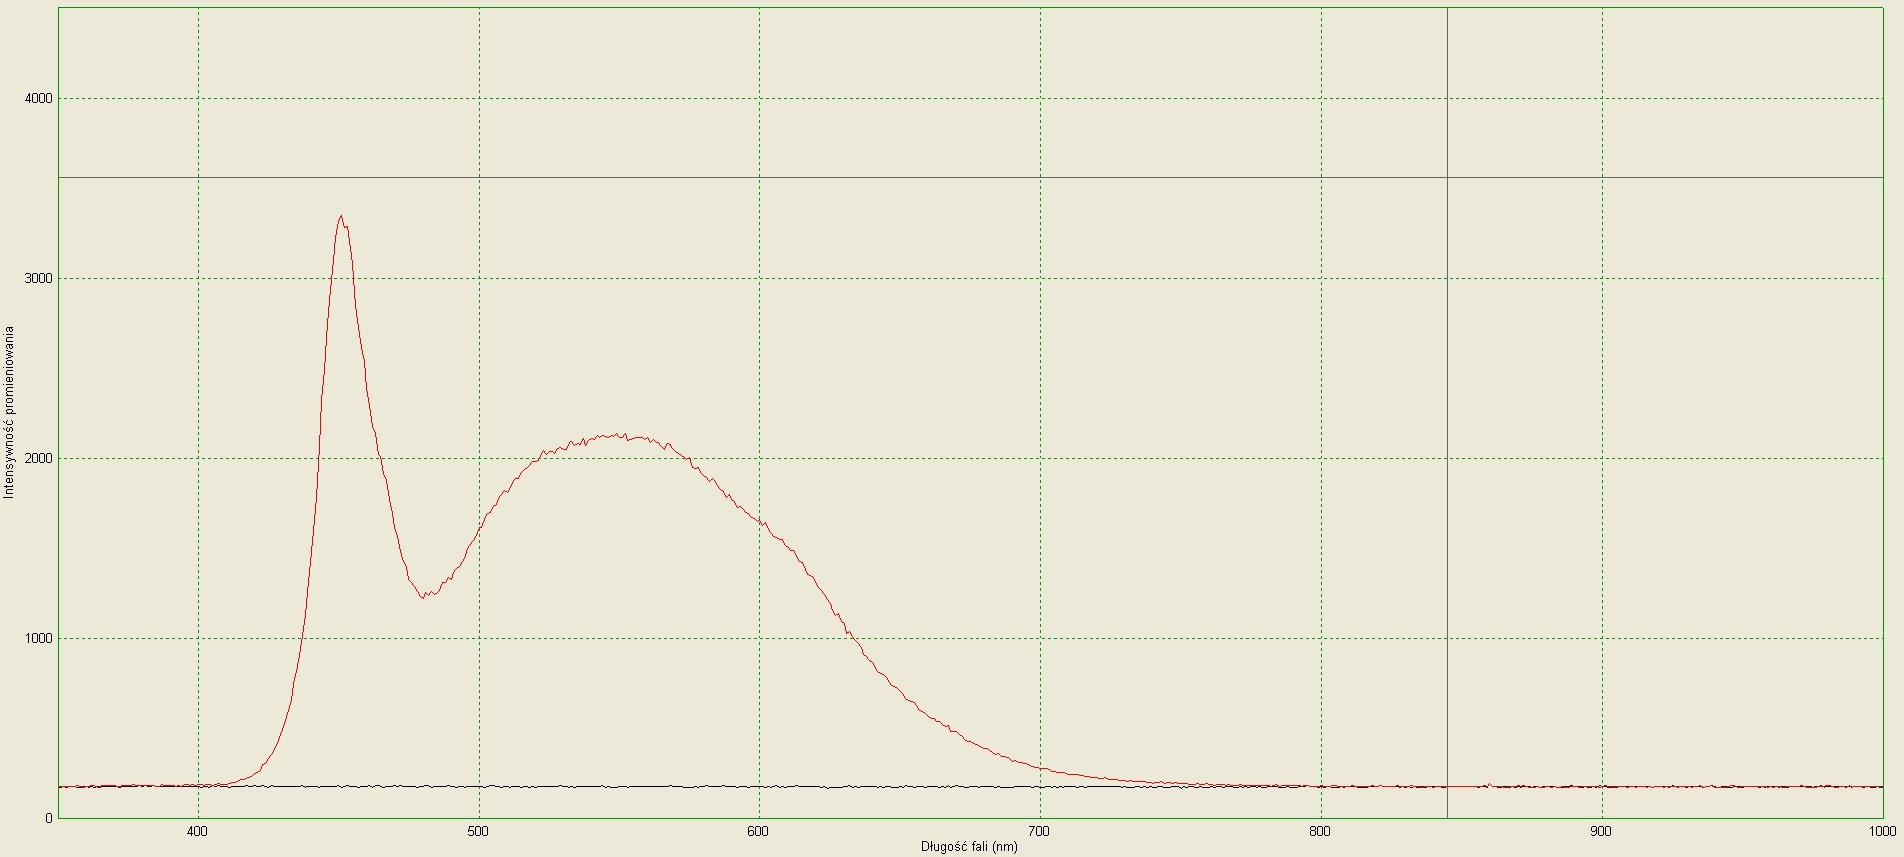
\includegraphics[width=\textwidth]{lampa2}
Widmo lampy 2.\\
\\

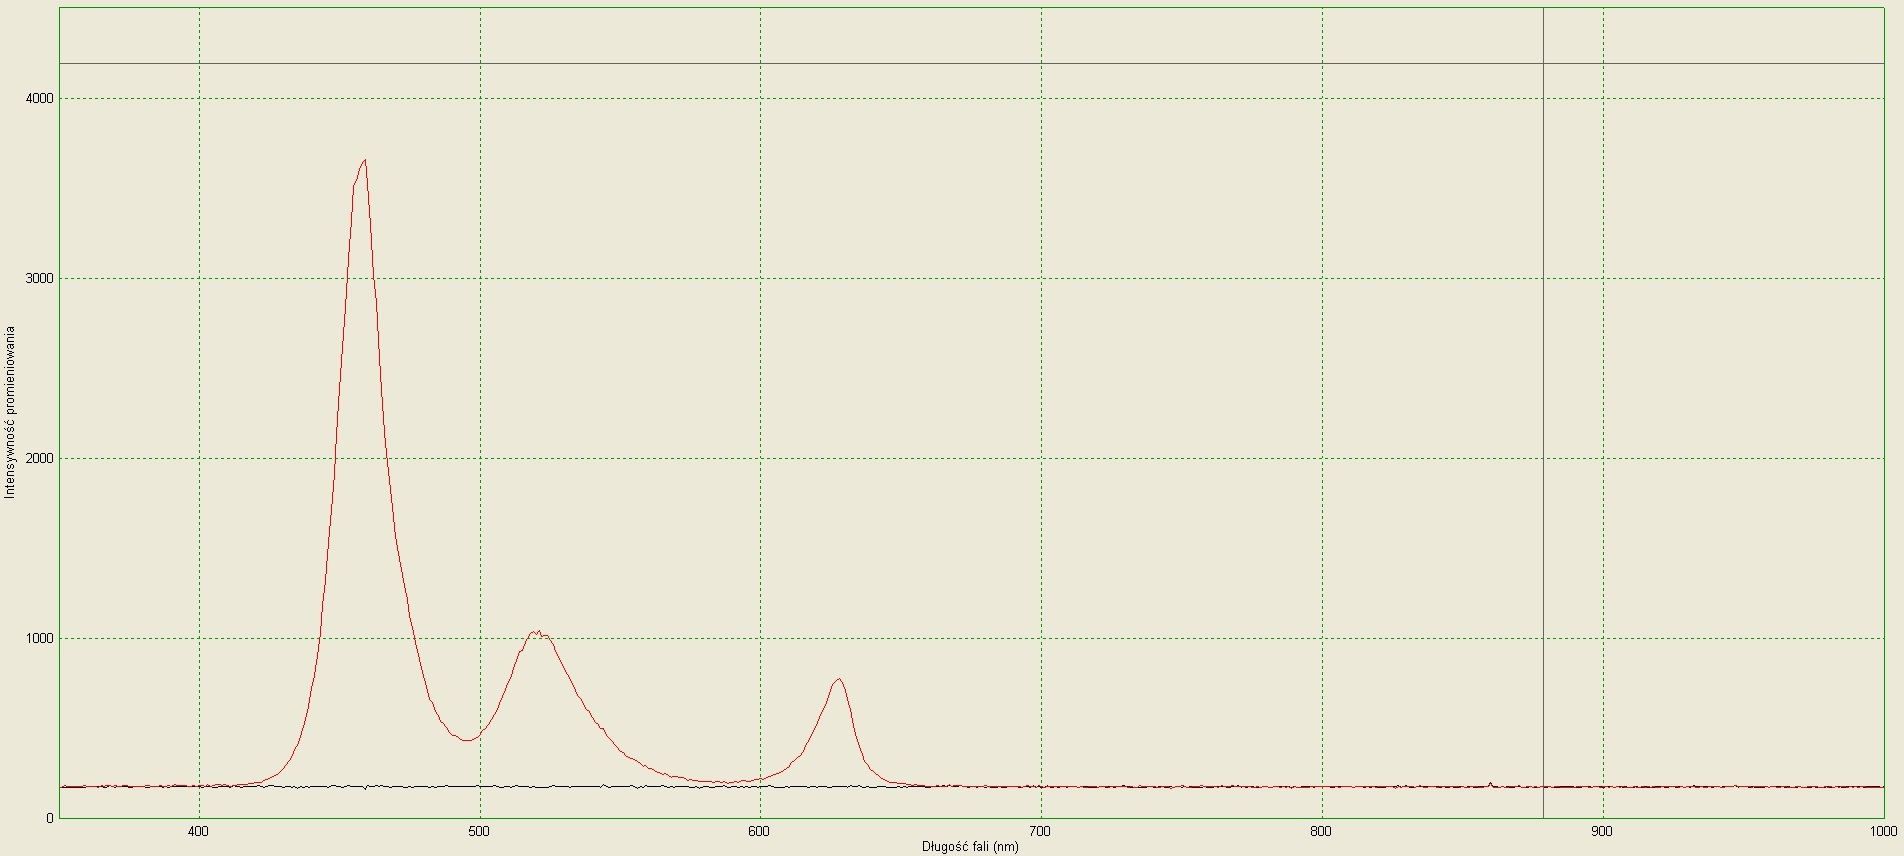
\includegraphics[width=\textwidth]{lampa3biale}
Widmo lampy 3. - światło białe\\
\\
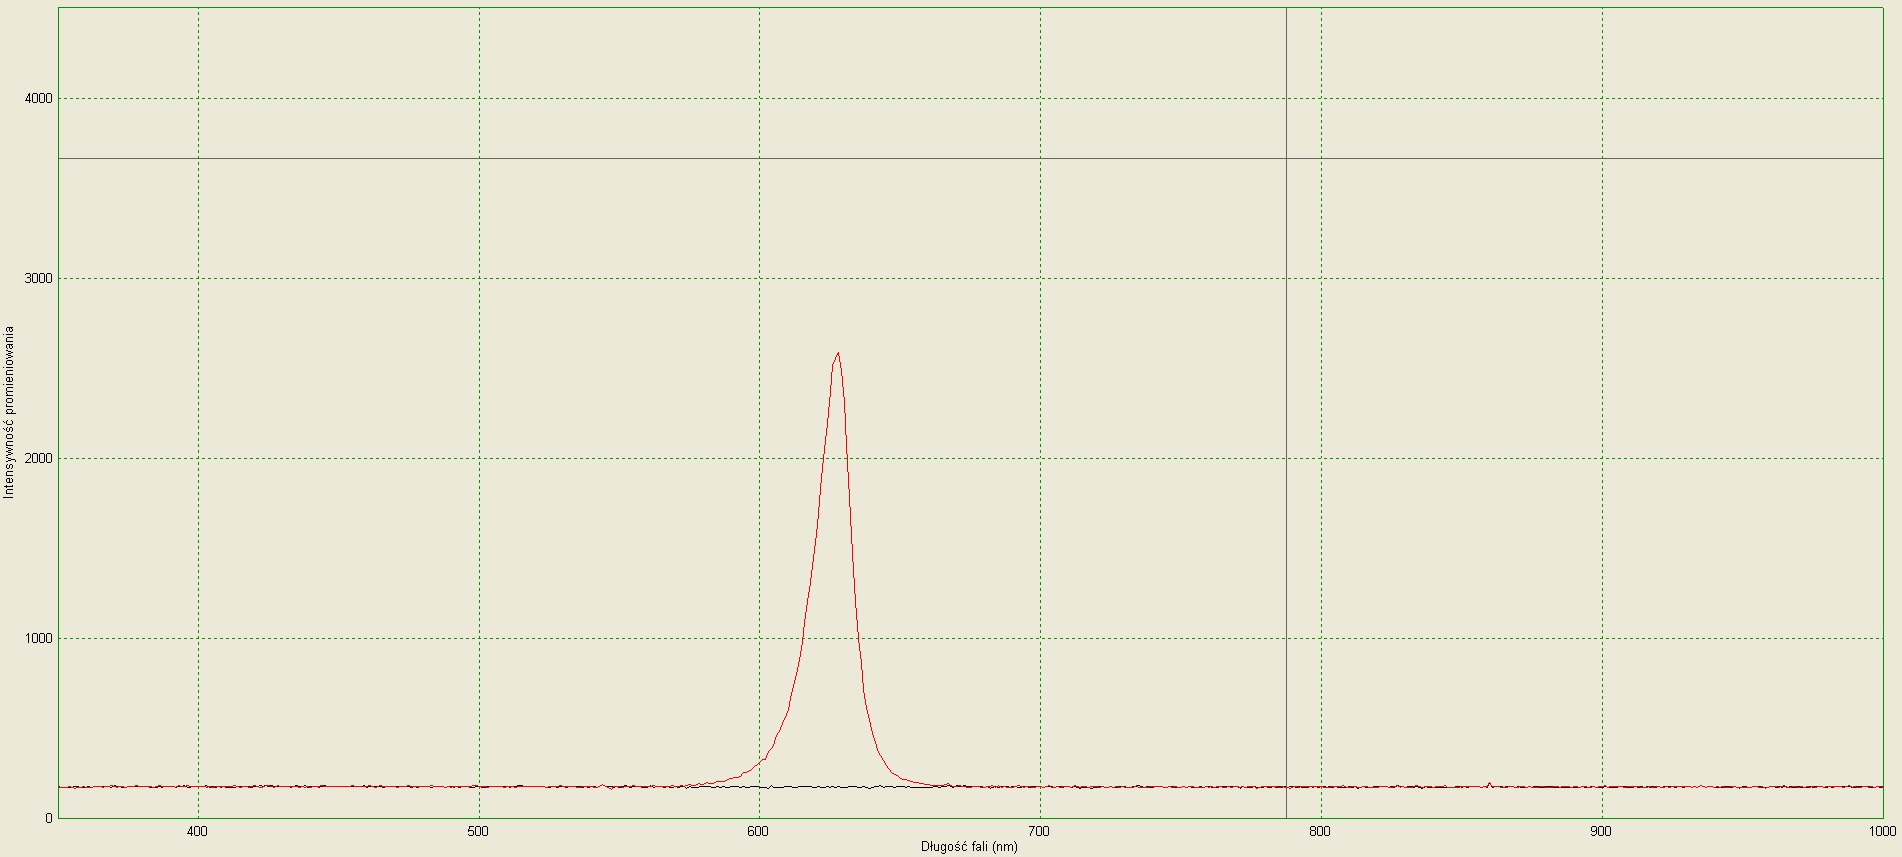
\includegraphics[width=\textwidth]{lampa3czerwone}
Widmo lampy 3. - światło czerwone\\
\\
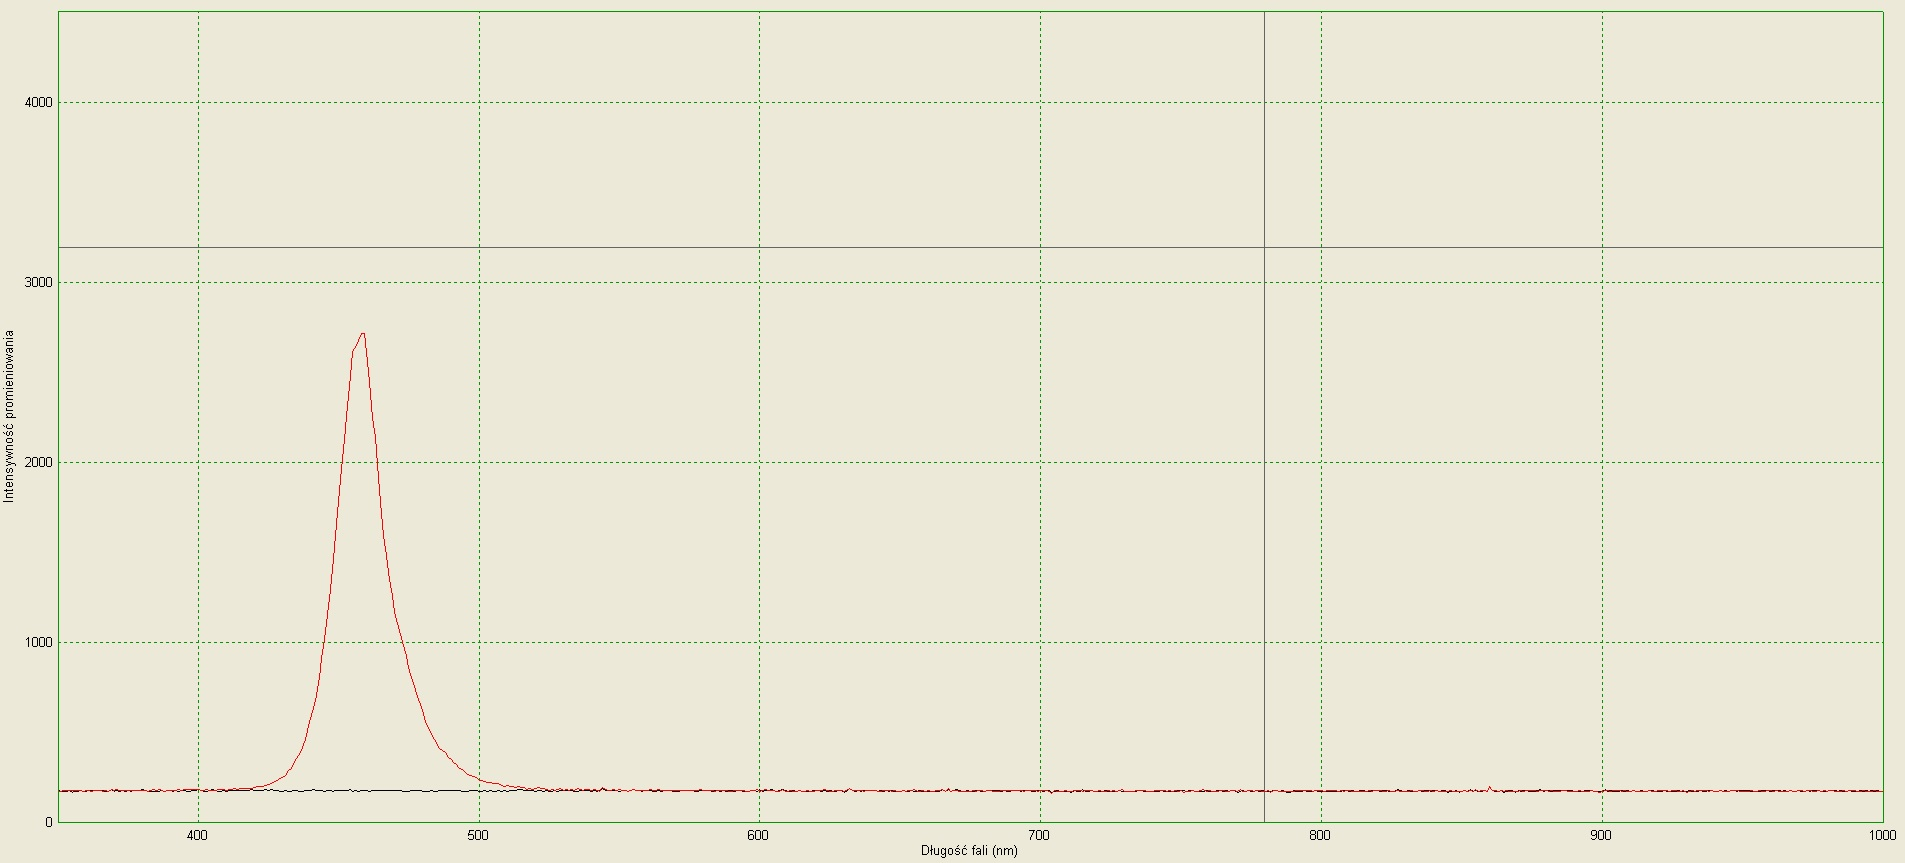
\includegraphics[width=\textwidth]{lampa3niebieskie}
Widmo lampy 3. - światło niebieskie\\
\\
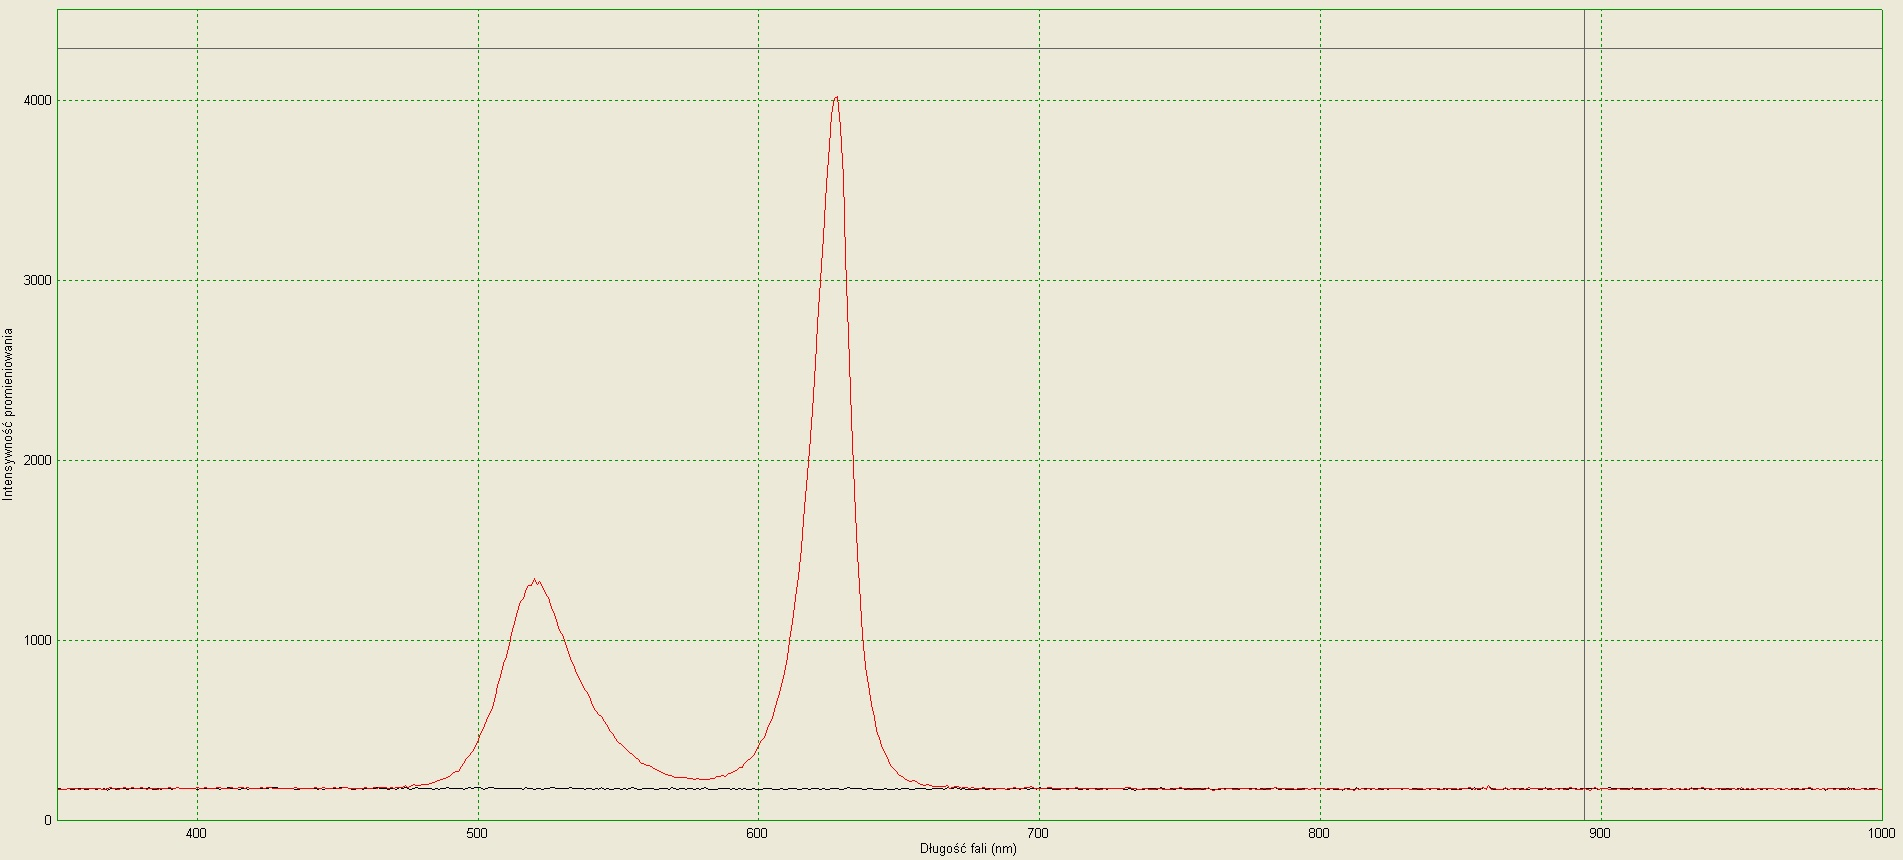
\includegraphics[width=\textwidth]{lampa3pomaranczowe}
Widmo lampy 3. - światło pomarańczowe\\
\\

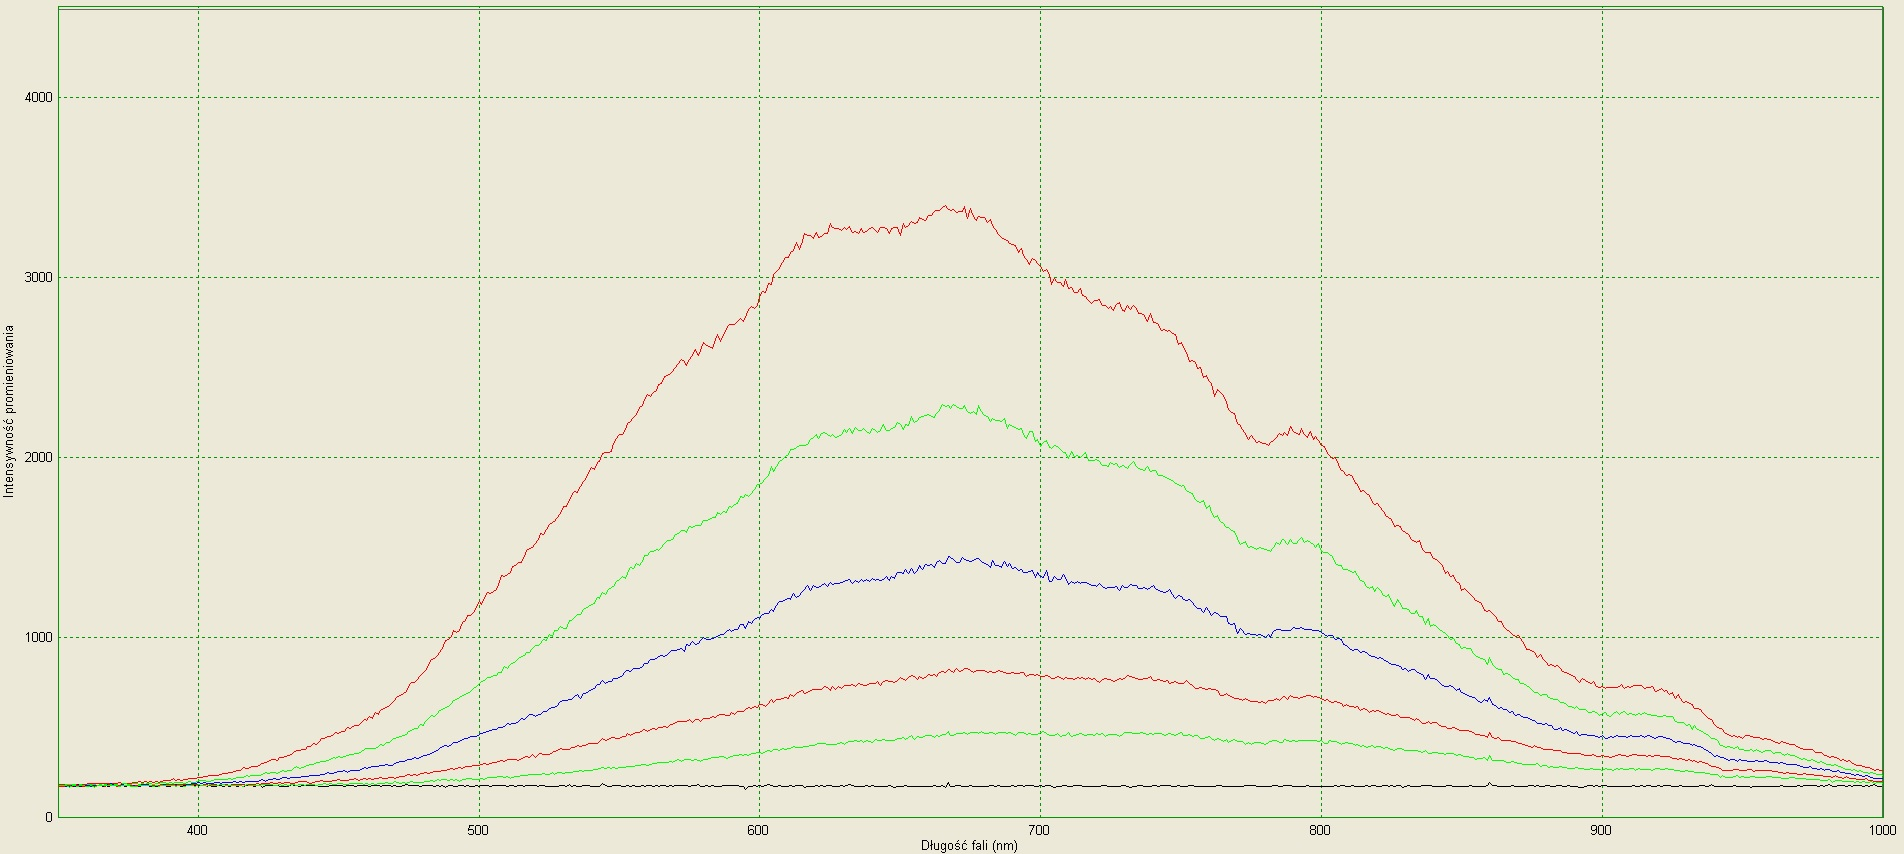
\includegraphics[width=\textwidth]{lampa4}
Widmo lampy 4. dla różnych natężeń prądu\\
\\

\newpage
\section*{Wnioski}
\forceindent Porównanie zapisanych widm z tablicami spektralnymi pokazuje, że w lampach A-C znajdują się następujące pierwiastki chemiczne :

\begin{center}
\begin{tabular}{|c|c|}
\hline
\textbf{Lampa} & \textbf{Pierwiastek} \\
\hline
A & Argon \\
\hline
B & Hel \\
\hline
C & Neon \\
\hline
\end{tabular}
\end{center}

\forceindent Jak widać na powyższych wykresach, maksymalne pasma spektralne dla lampy 1. położone są między $ 542,3 - 545,5 nm$ i $612,1 nm$, a dla lampy 2. w $459,0 nm$. Dla lampy 3. położenie pasm jest różne w zależności od koloru, zaś dla lampy 4. pasmo jest identyczne dla każdego natężenia prądu, zmienia się jedynie intensywność świecenia.\\

\forceindent Dodatkowo, po porównaniu widama lampy 1. z tablicą spektralną rtęci, można zauważyć, że intensywności dla odpowiednich długości fali, przedstawione w tabeli, bardzo dobrze pokrywają się z wykresem, co pokazuje, że pierwiastkiem emitującym światło w świetlówkach kompaktowych jest rtęć. \\

\forceindent Przeprowadzone doświadczenie unaocznia różnicę między różnymi rodzajami światła. Różnice te wynikają z tego, że różne żarówki wykonane są z różnych pierwiastków, co widać szczególnie w przypadku lamp A, B i C. Różnica w widmach wynika z różnic w długości fali światła wpadającego do spektrometru, co gołym okiem widać na przykładzie lampy 3., której różne barwy światła różniły się znacząco swoimi widmami. Doświadczenie wykorzystujące lampę 4. ukazuje, że intensywność świecenia, jak można było przewidzieć, nie wpłynie w sposób zauważalny na zakres pasma światła, zmieni się jedynie intensywność światła.

\end{document}
